% Options for packages loaded elsewhere
\PassOptionsToPackage{unicode}{hyperref}
\PassOptionsToPackage{hyphens}{url}
%
\documentclass[
]{article}
\usepackage{amsmath,amssymb}
\usepackage{iftex}
\ifPDFTeX
  \usepackage[T1]{fontenc}
  \usepackage[utf8]{inputenc}
  \usepackage{textcomp} % provide euro and other symbols
\else % if luatex or xetex
  \usepackage{unicode-math} % this also loads fontspec
  \defaultfontfeatures{Scale=MatchLowercase}
  \defaultfontfeatures[\rmfamily]{Ligatures=TeX,Scale=1}
\fi
\usepackage{lmodern}
\ifPDFTeX\else
  % xetex/luatex font selection
\fi
% Use upquote if available, for straight quotes in verbatim environments
\IfFileExists{upquote.sty}{\usepackage{upquote}}{}
\IfFileExists{microtype.sty}{% use microtype if available
  \usepackage[]{microtype}
  \UseMicrotypeSet[protrusion]{basicmath} % disable protrusion for tt fonts
}{}
\makeatletter
\@ifundefined{KOMAClassName}{% if non-KOMA class
  \IfFileExists{parskip.sty}{%
    \usepackage{parskip}
  }{% else
    \setlength{\parindent}{0pt}
    \setlength{\parskip}{6pt plus 2pt minus 1pt}}
}{% if KOMA class
  \KOMAoptions{parskip=half}}
\makeatother
\usepackage{xcolor}
\usepackage[margin=1in]{geometry}
\usepackage{graphicx}
\makeatletter
\def\maxwidth{\ifdim\Gin@nat@width>\linewidth\linewidth\else\Gin@nat@width\fi}
\def\maxheight{\ifdim\Gin@nat@height>\textheight\textheight\else\Gin@nat@height\fi}
\makeatother
% Scale images if necessary, so that they will not overflow the page
% margins by default, and it is still possible to overwrite the defaults
% using explicit options in \includegraphics[width, height, ...]{}
\setkeys{Gin}{width=\maxwidth,height=\maxheight,keepaspectratio}
% Set default figure placement to htbp
\makeatletter
\def\fps@figure{htbp}
\makeatother
\setlength{\emergencystretch}{3em} % prevent overfull lines
\providecommand{\tightlist}{%
  \setlength{\itemsep}{0pt}\setlength{\parskip}{0pt}}
\setcounter{secnumdepth}{-\maxdimen} % remove section numbering
\ifLuaTeX
  \usepackage{selnolig}  % disable illegal ligatures
\fi
\IfFileExists{bookmark.sty}{\usepackage{bookmark}}{\usepackage{hyperref}}
\IfFileExists{xurl.sty}{\usepackage{xurl}}{} % add URL line breaks if available
\urlstyle{same}
\hypersetup{
  hidelinks,
  pdfcreator={LaTeX via pandoc}}

\author{}
\date{\vspace{-2.5em}}

\begin{document}

\hypertarget{methods}{%
\section{Methods}\label{methods}}

\vspace{0.5cm}

\hypertarget{a-mesocosm-design}{%
\subsection{(a) Mesocosm Design}\label{a-mesocosm-design}}

~~~~~The Silbiger Lab mesocosm system at California State University,
Northridge was used to emulate experimental conditions of a semi-diurnal
tidal fluctuation across a gradient of temperatures and blocked exposure
to either low or high pH. The facility operated as a closed-loop system,
wherein water from individual tanks was continuously recirculated back
into a central holding reservoir (sump). Unbuffered natural seawater was
collected from the Southern California Marine Institute (SCMI) in San
Pedro, CA and filtered through three mesh filters (20 \(\mu\)m, 5
\(\mu\)m, 1 \(\mu\)m) prior to being introduced into the sump of the
mesocosm system. Within the system, recirculating seawater underwent
further filtration through three 50 \(\mu\)m carbon bag filters, eight
mesh filters, a UV sterilizer (Comet Series 95 Watt Lamp), and a chiller
(Aqua Logic Delta Star, DS-4) which maintained water quality and chilled
seawater to ambient conditions. Weekly water replacements, accounting
for approximately 50\% of the total volume, were conducted to prevent
the accumulation of metabolic waste and to maintain stable carbonate
parameters within the system. The mesocosm system was equipped with 16
experimental tanks (53.9 cm (L) x 31.75 cm (W) x 34.29cm (H)) with
individual controls for temperature, light intensity, and water flow.
Each tank was outfitted with a submersible powerhead pump (Hydor Nano
Koralina 240 powerhead, 240 GPH), 200 W Heater (Hydor aquarium heater),
temperature probe (Neptune Systems, \(\pm\) 0.1\(^\circ\)C), pH probe
(Neptune Systems, Lab Grade Double Junction, measures pH from 4.0 to
12.0 \(\pm\) 0.1), three flow sensors (Apex, FS25 \(\frac{1}{4}\)''
fitting, flow rates from 3-12 GPH (12-24 LP)), and a temperature logger
(HOBO TidBit MX2203, \(\pm\) 0.2\(^\circ\)C). LED lights (Halo Basic
M-110) in each tank followed a 12:12 day/night cycle, which mimicked the
local light conditions using a sunset and sunrise table.

~~~~~Each individual tank was programmed to experience tidal
fluctuations as well as temperature/pH controlled seawater conditions
for their respective treatments. Programmable solenoid valves (Apex
Neptune) were utilized to adjust the seawater flow rates to each tank,
ensuring that either inflow rates exceeded outflow drain rates
simulating a high tide condition or outflow drain rates exceeded inflow
rates to simulate a low tide condition. This emulation aimed to
replicate the semi-diurnal tidal characteristic of the Pacific Coast.
Within a 24-hour period, two high tide and two low tide fluctuations,
each lasting six hours, were generated by either opening or closing the
solenoids. Flow rates were meticulously maintained on a daily basis
using a graduated cylinder and timepiece to ensure a programmable inflow
of 10 L/h, constant total inflow of 10 L/hour, and a constant outflow
drain rate of 15 L/hour, thereby creating the desired tidal effect.
Precise control over temperature in each tank was achieved by employing
a programmable thermostat (Neptune Apex), which automatically activated
or deactivated heaters in response to temperature deviations from the
set range. Individual tank pH levels were regulated using a pH-stat
set-up through the direct bubbling and mixing of CO2 facilitated by a pH
logger and solenoid valves (Neptune system) attached to a CO2 tank
(PhosBan Reactor 150). Additionally, in each tank, a venturi connected
to an aquarium pump facilitated the mixing of ambient air to stabilize
the pH levels in the treatment tanks. After recirculation into the sump
system, the sweater was chilled to ambient condition and scrubbed of CO2
using a phosban reactor (Phosban 150 Reactor).

~~~~~Throughout the experiment, various water quality parameters were
regularly measured to monitor environmental conditions within the tanks.
pH, dissolved oxygen (DO), and temperature were assessed daily at
consistent times to ensure accurate readings and facilitate the
calibration of in-tank temperature probes for precise measurements. pH
and dissolved oxygen levels were measured daily, within each tank using
a Termo Specific ORION ISE instrument with a resolution of 0.1 mV and an
accuracy of \(\pm\) 0.2 mV or \(\pm\) 0.05\%. Simultaneously,
temperature readings were obtained using a Thermo Fisher Trace digital
thermometer. The temperature data also aided in calibrating the
thermostat sensors within each tank, which were adjusted once a day to
maintain accurate temperature control. pH on the total scale was
calculated from mV and temperature by using a multipoint calibration to
a tris standard solution from the Dickson Lab at Scripps Institution of
Oceanography following Dickson SOP 6a \citep{dickson2007guide}. Accuracy
of the pH was tested against a Tris buffer of known pH from the Dickson
Lab at Scripps Institution of Oceanography \citep{dickson2007guide}. The
pH values for the individual aquaria were calculated using the seacarb
package in R, accounting for temperature corrections specific to each
tank \citep{gattuso2015package}. I also measured total alkalinity (TA)
from water samples collected once every few days (3-4 days) from each
experimental tank and sump. All total alkalinity (TA) water samples were
collected and stored in 125 ml Nalgene containers. Prior to use, these
containers underwent thorough cleaning in a 10\% HCl bath for 24 hours,
followed by rinsing with deionized (DI) water. Additionally, during
sample collection, the containers were rinsed three times with sample
water to ensure a representative water quality sample. Collected samples
were analyzed within 24 hours of collection using a T-5 automatic
titrator (Mettler Toledo) following the best practices for ocean CO2
measurements \citep{dickson2007guide}. To verify accuracy, a certified
reference material (Reference Material for Oceanic CO2 Measurements, A.
Dickson, Scripps Institution of Oceanography) was run prior to each
total alkalinity measurement with an error no greater than 1.0\% off
from the certified value \citep{dickson2007guide}.

\begin{table}[!ht]
    \centering
    \begin{tabular}{|c|c|c|c|c|c|}
    \hline
        \textbf{Set Temp} & \textbf{pH Treatment} & \textbf{Mean Temp C} & \textbf{Mean pH} & \textbf{Mean Salinity} & \textbf{Mean DO \%} \\ \hline
        10 & Sump & 10.94 ± 0.26 & 7.92 ± 0.04 & 32.32 ± 0.37 & 114.82 ± 1.09 \\ \hline
        12 & Ambient & 12.91 ± 0.2 & 7.95 ± 0.02 & 33.24 ± 0.11 & 113.68 ± 1.59 \\ \hline
        12 & Low & 13.17 ± 0.41 & 7.71 ± 0.03 & 32.85 ± 0.15 & 112.37 ± 1.37 \\ \hline
        14 & Ambient & 13.9 ± 0.1 & 7.97 ± 0.02 & 32.93 ± 0.07 & 106.18 ± 1.08 \\ \hline
        14 & Low & 13.7 ± 0.22 & 7.67 ± 0.01 & 32.88 ± 0.09 & 119.31 ± 2.79 \\ \hline
        16 & Ambient & 16.17 ± 0.13 & 7.93 ± 0.02 & 32.91 ± 0.07 & 102.32 ± 1.01 \\ \hline
        16 & Low & 15.92 ± 0.32 & 7.69 ± 0.02 & 32.9 ± 0.07 & 104.81 ± 6.25 \\ \hline
        18 & Ambient & 18.18 ± 0.24 & 7.91 ± 0.02 & 32.94 ± 0.07 & 99.78 ± 1.05 \\ \hline
        18 & Low & 18.38 ± 0.26 & 7.68 ± 0.02 & 32.92 ± 0.05 & 98.79 ± 1.68 \\ \hline
        20 & Ambient & 20.76 ± 0.31 & 7.87 ± 0.04 & 32.82 ± 0.07 & 103.31 ± 1.07 \\ \hline
        20 & Low & 19.62 ± 0.57 & 7.64 ± 0.02 & 32.95 ± 0.08 & 96.02 ± 5.38 \\ \hline
        22 & Ambient & 22.36 ± 0.39 & 7.84 ± 0.02 & 32.96 ± 0.07 & 98.98 ± 0.77 \\ \hline
        22 & Low & 21.64 ± 0.49 & 7.69 ± 0.01 & 32.92 ± 0.08 & 96.65 ± 1.26 \\ \hline
        24 & Ambient & 24.75 ± 0.59 & 7.82 ± 0.03 & 32.76 ± 0.13 & 102.56 ± 1.28 \\ \hline
        24 & Low & 22.88 ± 0.66 & 7.69 ± 0.02 & 32.68 ± 0.09 & 100.09 ± 1.32 \\ \hline
        26 & Ambient & 24.45 ± 1 & 7.89 ± 0.02 & 32.85 ± 0.18 & 98.99 ± 2.1 \\ \hline
        26 & Low & 25.52 ± 0.77 & 7.66 ± 0.02 & 32.99 ± 0.06 & 92.3 ± 1.59 \\ \hline
    \end{tabular}
    \caption{Table 1. Summary statistics (mean$\pm$sd) for tank treatments and associated water quality parameters subjected to low and ambient pH levels alongside temperature variations ranging from 12-26$^\circ$C. Error bars depict standard deviations, providing insights into the variability within each treatment group. The depicted parameters include temperature treatment, pH treatment, mean temperature (°C), mean pH, mean salinity, mean dissolved oxygen percentage}
    \label{meso-stat-summary}
\end{table}

\begin{table}[!ht]
    \centering
    \begin{tabular}{|c|c|c|c|c|c|c|}
    \hline
        \textbf{Set Temp} & \textbf{pH Treatment} & \textbf{Mean TA} & \textbf{Mean pCO2} & \textbf{Mean HCO3} & \textbf{Mean CO3} & \textbf{Mean DIC} \\ \hline
        10 & Sump & 2328.01 ± 25.92 & 4978230.96 ± 275963.47 & 20.26 ± 0.29 & 1.07 ± 0.06 & 21.61 ± 0.29 \\ \hline
        12 & Ambient & 2358.28 ± 19.58 & 4920188.24 ± 223654.68 & 19.13 ± 0.21 & 1.12 ± 0.04 & 20.45 ± 0.2 \\ \hline
        12 & Low & 2359.61 ± 18.06 & 4628623.06 ± 341408.31 & 10.04 ± 0.07 & 0.35 ± 0.03 & 10.58 ± 0.08 \\ \hline
        14 & Ambient & 2357.76 ± 17.16 & 2711089.29 ± 142579.38 & 10.69 ± 0.1 & 0.68 ± 0.03 & 11.49 ± 0.09 \\ \hline
        14 & Low & 2376.31 ± 22.23 & 649410.85 ± 24204.31 & 1.28 ± 0.01 & 0.04 ± 0 & 1.34 ± 0.01 \\ \hline
        16 & Ambient & 2355.87 ± 19.49 & 3363571.87 ± 164547.58 & 11.88 ± 0.11 & 0.75 ± 0.03 & 12.76 ± 0.11 \\ \hline
        16 & Low & 2350.55 ± 21.16 & 1242533.16 ± 55051.05 & 2.5 ± 0.03 & 0.09 ± 0 & 2.64 ± 0.03 \\ \hline
        18 & Ambient & 2360.54 ± 18.2 & 3843319.75 ± 202604.37 & 13.02 ± 0.12 & 0.86 ± 0.04 & 14.02 ± 0.11 \\ \hline
        18 & Low & 2409.62 ± 18.07 & 1947471.11 ± 91567.08 & 3.83 ± 0.03 & 0.15 ± 0.01 & 4.04 ± 0.03 \\ \hline
        20 & Ambient & 2348.58 ± 21.84 & 4412288.41 ± 316379.33 & 14.07 ± 0.21 & 0.96 ± 0.06 & 15.21 ± 0.2 \\ \hline
        20 & Low & 2358.68 ± 17.84 & 2840268.86 ± 137486.09 & 5.01 ± 0.04 & 0.18 ± 0.01 & 5.29 ± 0.04 \\ \hline
        22 & Ambient & 2369.09 ± 19.13 & 5298578.58 ± 240316.39 & 15.42 ± 0.13 & 1.02 ± 0.04 & 16.62 ± 0.13 \\ \hline
        22 & Low & 2358.77 ± 16.72 & 3099996.23 ± 119715.11 & 6.17 ± 0.04 & 0.28 ± 0.01 & 6.54 ± 0.05 \\ \hline
        24 & Ambient & 2356.82 ± 21.89 & 6031162.38 ± 439328.11 & 16.43 ± 0.23 & 1.14 ± 0.07 & 17.76 ± 0.21 \\ \hline
        24 & Low & 2367.69 ± 17.4 & 3745464.62 ± 190122.17 & 7.39 ± 0.05 & 0.35 ± 0.02 & 7.85 ± 0.06 \\ \hline
        26 & Ambient & 2362.64 ± 19.05 & 5523863.5 ± 327978.24 & 17.35 ± 0.23 & 1.36 ± 0.06 & 18.88 ± 0.2 \\ \hline
        26 & Low & 2350.6 ± 20.16 & 4640263.18 ± 268033.32 & 8.52 ± 0.09 & 0.42 ± 0.02 & 9.08 ± 0.09 \\ \hline
    \end{tabular}
    \caption{Table 2. Summary statistics (mean$\pm$sd) for tank treatments and associated seawater carbonate chemistry parameters subjected to low and ambient pH levels alongside temperature variations ranging from 12-26$^\circ$C. Error bars depict standard deviations, providing insights into the variability within each treatment group. The depicted parameters include mean total alkalinity (TA), mean partial pressure of CO2 (pCO2), mean bicarbonate concentration (HCO3), mean carbonate concentration (CO3), and mean dissolved inorganic carbon (DIC) computed using the seacarb package in R \citep{gattuso2015package}.}
    \label{carbonate-stat-summary}
\end{table}

\hypertarget{b-species-collection-and-maintenance}{%
\subsection{(b) Species Collection and
Maintenance}\label{b-species-collection-and-maintenance}}

\begin{figure}[htbp]
    \centering
    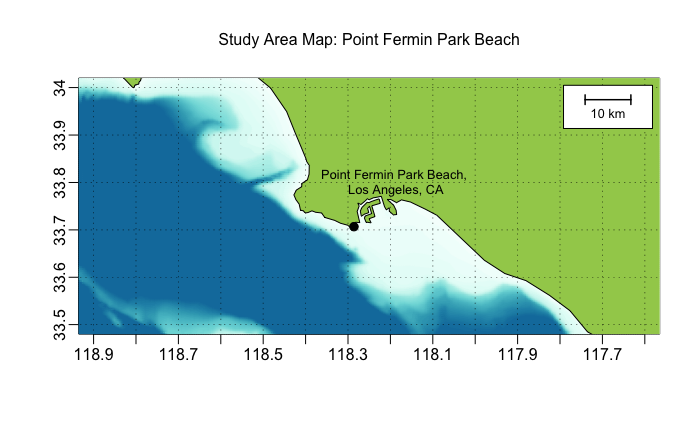
\includegraphics[width=1\textwidth]{Images/map.png}
    \caption{Figure 2. Map for study site collection located at Point Fermin State Beach (coordinates: latitude 33.7056° N, longitude 118.2935° W). Created using the Oce package \citep{kelley2018oce}.}
    \label{fig:study-site-map}
\end{figure}

~~~~~ For this experiment, black turban snails
(\emph{Tegula funebralis}) (N=80 individuals) were collected haphazardly
from tidepools in Point Fermin, San Pedro, CA (Figure 2.) on August 16,
2022 (SCP ID: S-220520002-22054-001). All collections were made and
transported during low tide to minimize any physiological variation that
might be related to endogenous tidal rhythms. Individuals of
\emph{T. funebralis} were measured for shell width (dorsal to ventral)
between 18-22 mm using Vernier calipers, since shell height is a
reliable predictor for body mass. Organisms were then transported back
to California State University, Northridge in a wet insulated container
where they were measured for blotted wet mass (g), volume displacement
(mL), shell height (mm), and shell width (mm) and tagged using a
previously weighed FloyTag placed at the apex of the dorsal side of the
shell with coraffix glue. The snails were then randomized and assigned
to an experimental treatment as detailed below. Each snail was randomly
assigned to one of 16 experimental aquaria across a range of 8
temperatures from 12-26\(^\circ\)C and two pH treatments, and placed
into their respective experimental tanks (n=4 per treatment). To adjust
the snails to their treatment temperatures, all snails started in
ambient temperature conditions (16\(^\circ\)C), and temperatures were
then increased or decreased at a rate of up to 2\(^\circ\) C per day
until reaching the set treatment temperature. The changes in pH for the
acidification treatments were simultaneously reduced with temperature
changes at a rate of up to \textasciitilde0.5 units per day during this
period as this is the fluctuation of pH that organisms in the intertidal
experience in a single day \citep{jellison2016ocean}. Organisms were
adjusted to experimental conditions for a week before the experiment
began. Throughout the experiment, snails were fed giant kelp wrack
\emph{Macrosystis pyrifera}, a highly preferred food, was collected from
Point Fermin, CA to feed organisms and placed on 3 inch PVC disks every
three days throughout the experiment. \emph{M. pyrifera} was rinsed with
fresh water to remove epiphytes prior to feeding.

\hypertarget{c-temperature-and-ph-treatment}{%
\subsection{(c) Temperature and pH
Treatment}\label{c-temperature-and-ph-treatment}}

\begin{figure}[htbp]
  \centering
  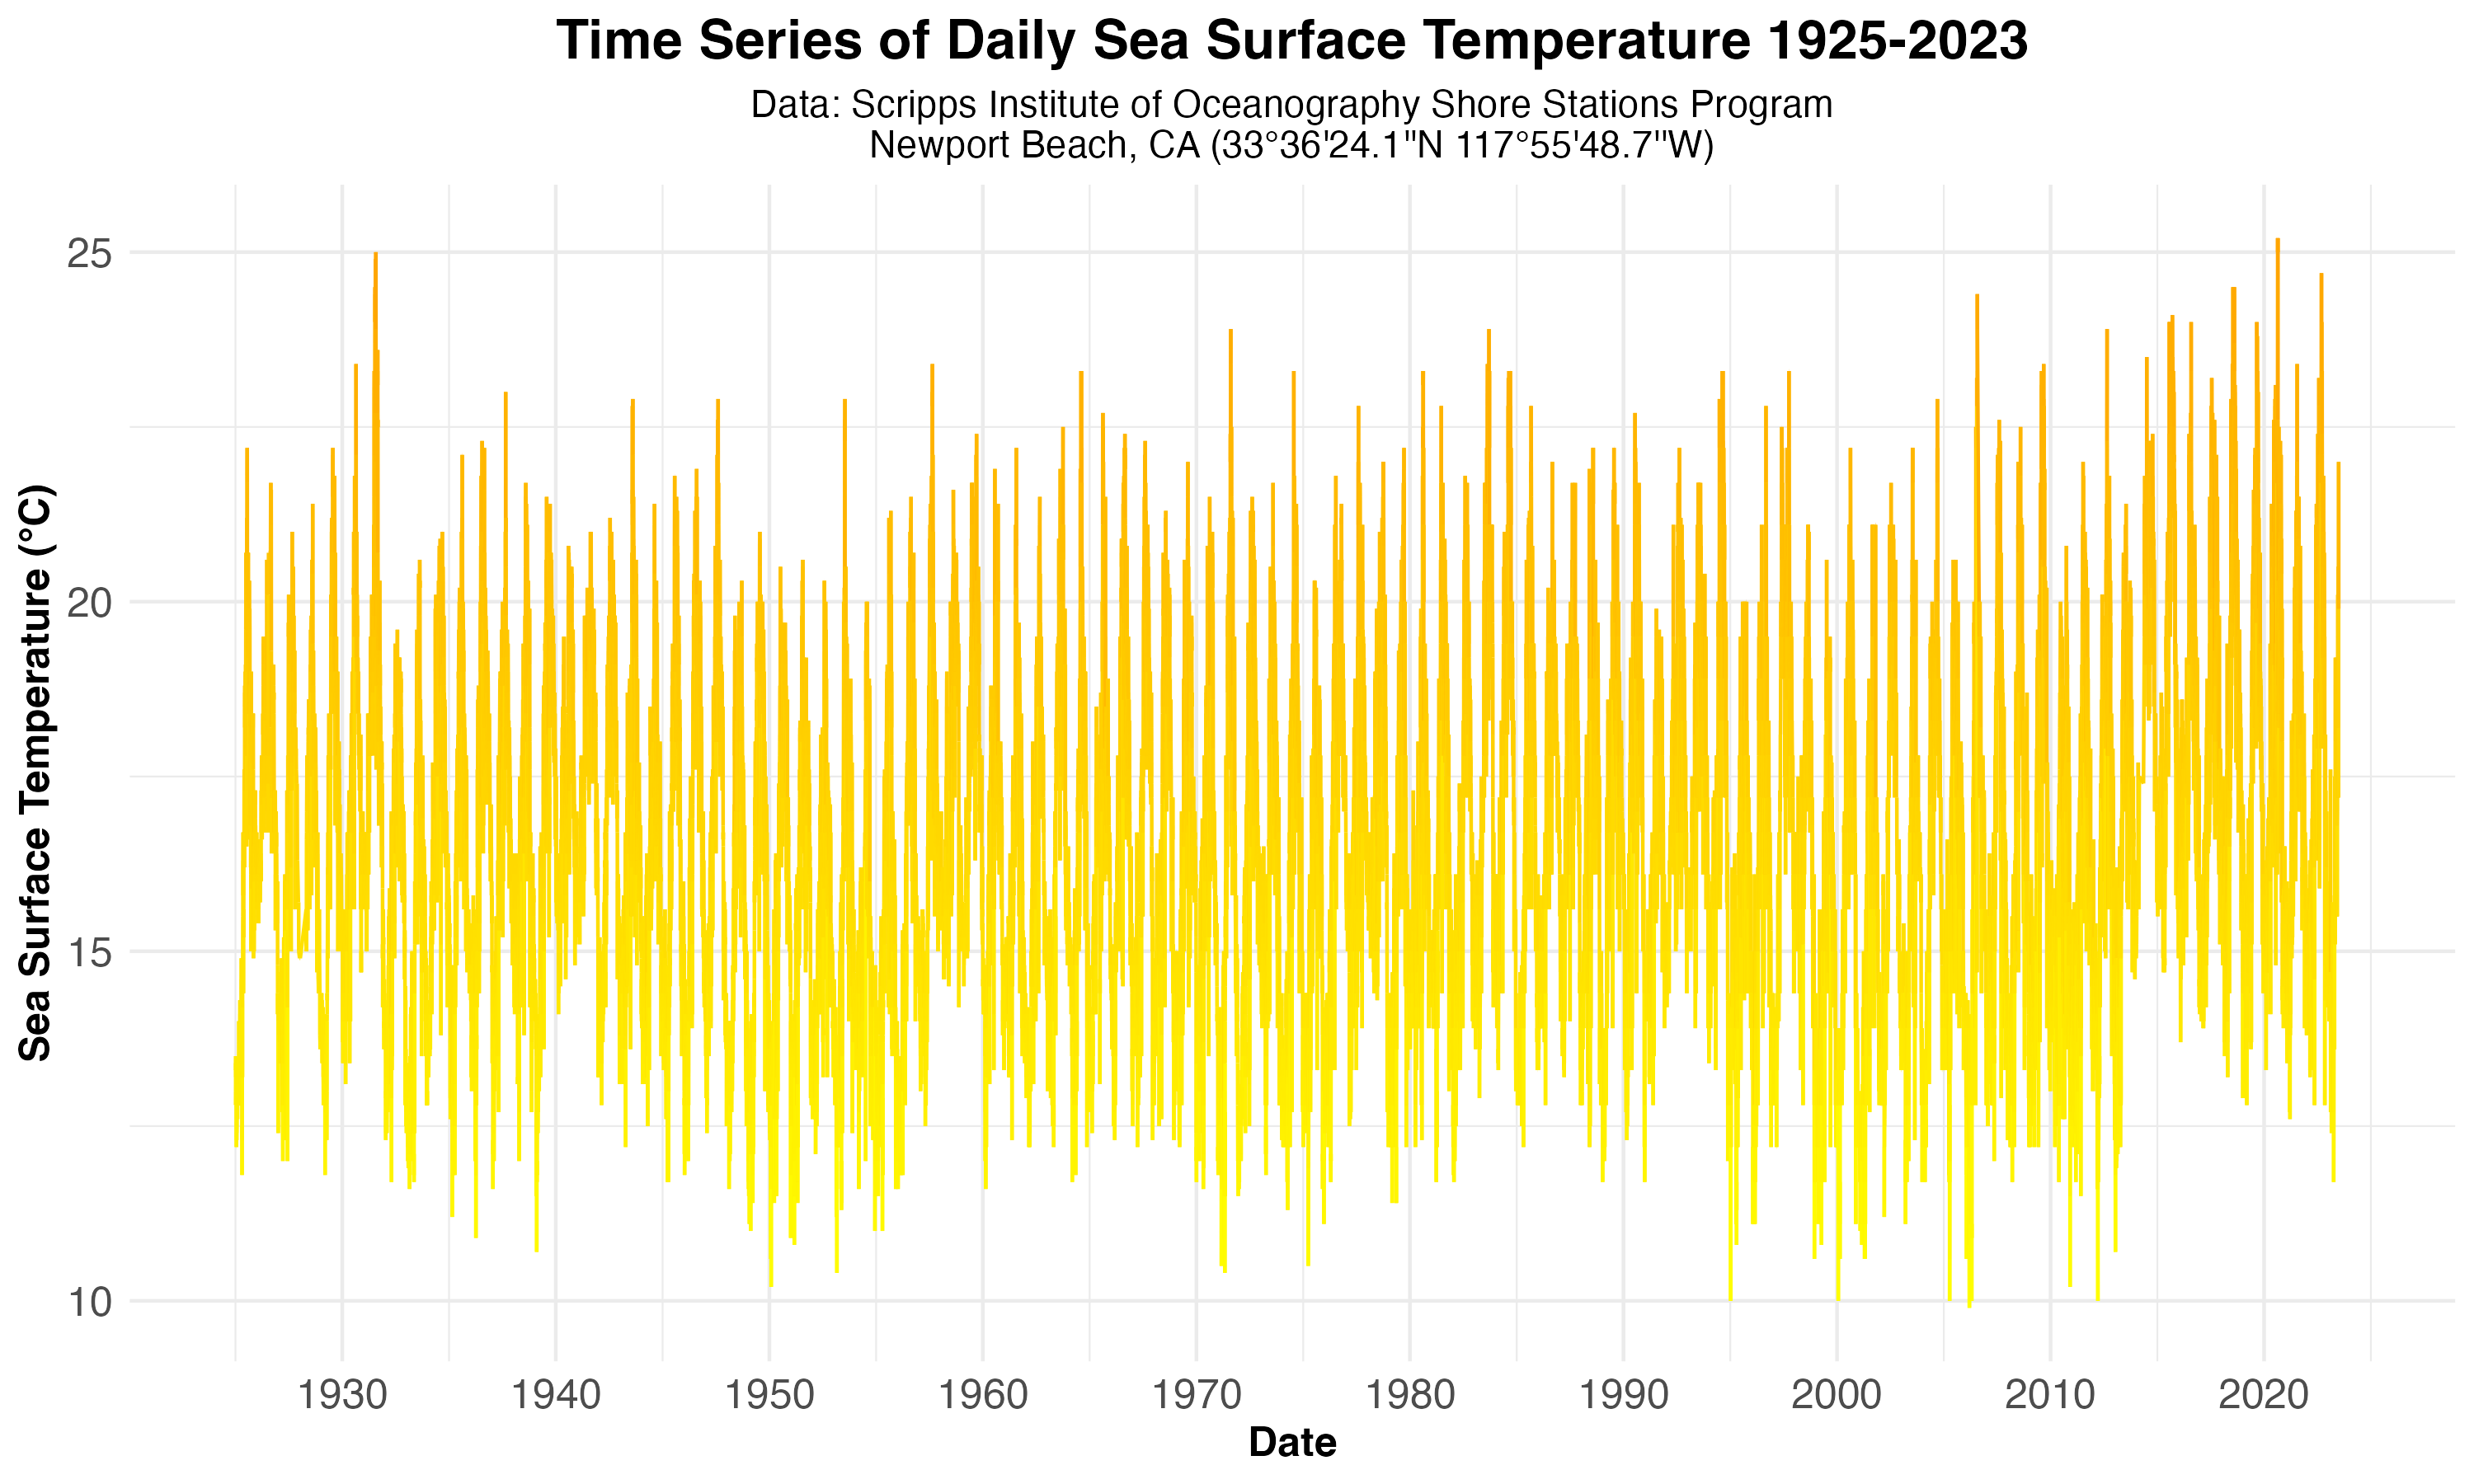
\includegraphics[width=0.8\textwidth]{Images/SST_timeseries_plot.png}
  \caption{Time series depicting the surface water sea surface temperature (SST) recorded from 1925 to 2023 at Newport Beach Pier in Newport, CA. The data were continuously collected, providing a visual representation of the daily surface temperature fluctuations near the study site. Data sourced from the UCSD Shore Stations Program \citep{carter2022shore}.}
  \label{fig:sst-timeseries}
\end{figure}

\begin{figure}[htbp]
  \centering
  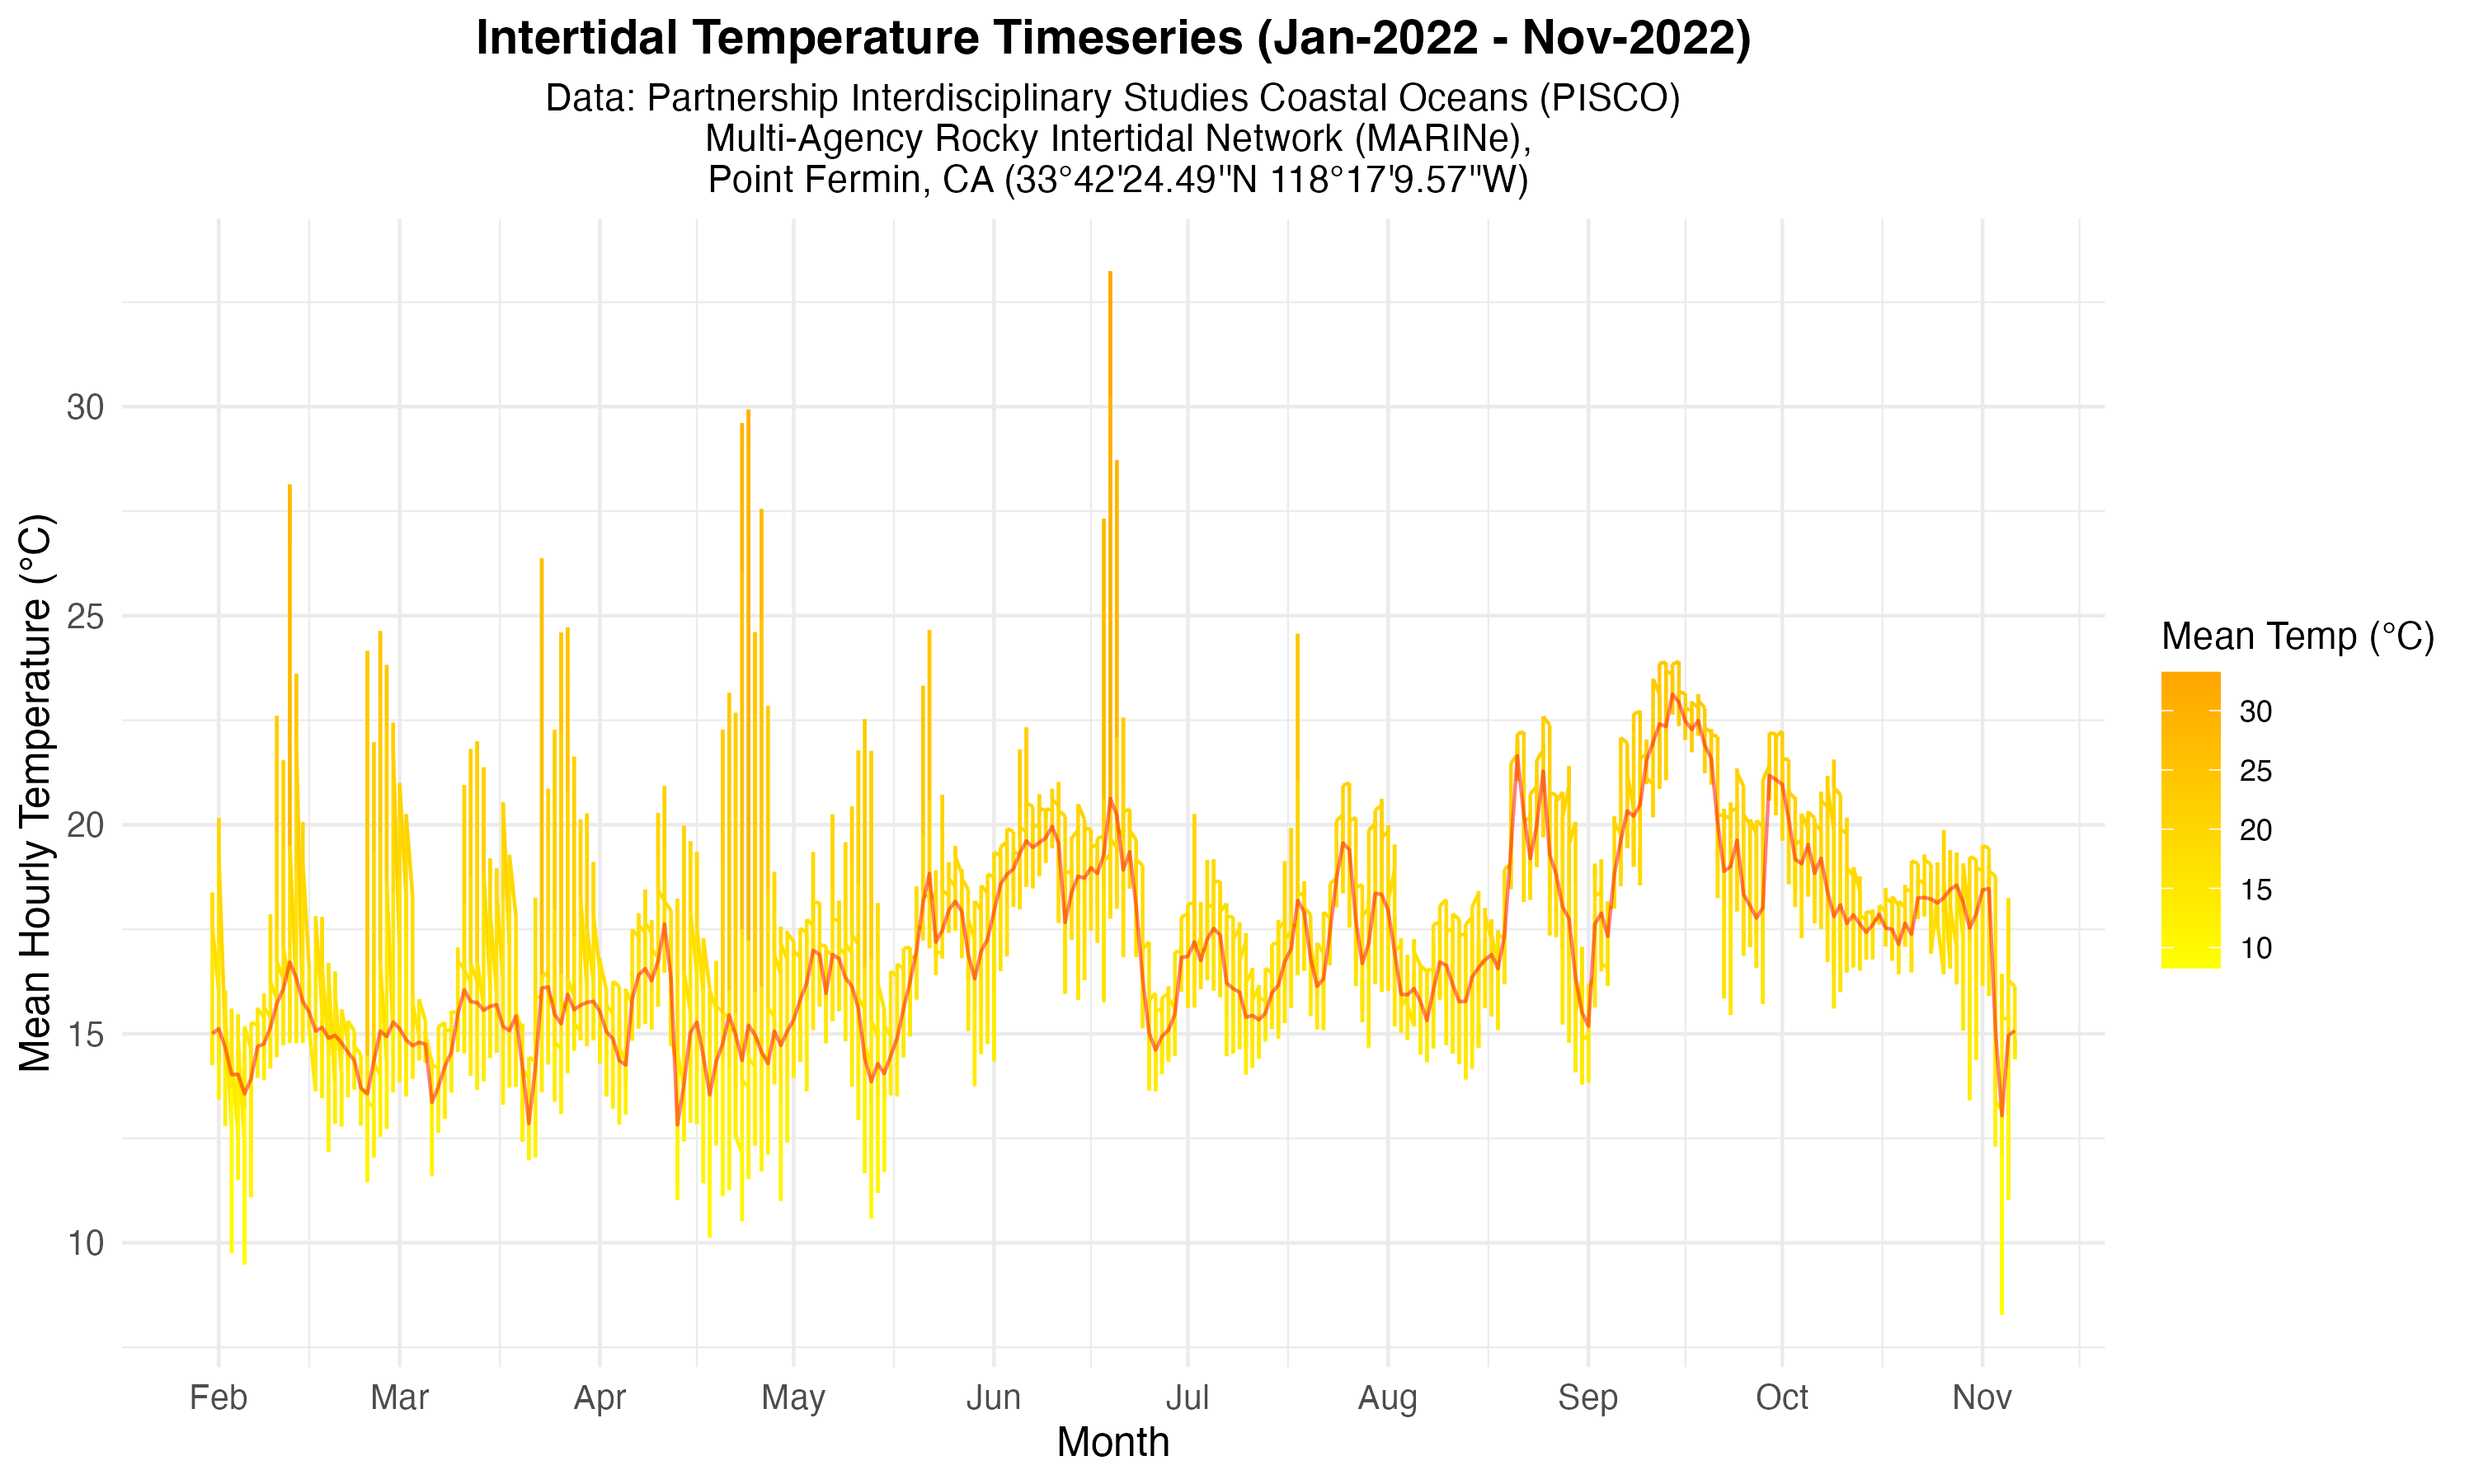
\includegraphics[width=0.8\textwidth]{Images/intertidal_timeseries_plot.png}
  \caption{Intertidal Temperature for Point Fermin, California (Data Collected Using: Onset Tidbit V2 Temp Data Logger). This figure illustrates temperature data collected from the intertidal mid zone using Onset Tidbit V2 Temp Data Logger, covering the period from January 2022 to November 2022. Data sourced from the Multi-Agency Rocky Intertidal Network (MARINe) and Partnership Interdisciplinary Studies Coastal Oceans for of (PISCO). \citep{marine_pisco_burnaford_2023}}
  \label{fig:intertidal-timeseries}
\end{figure}

\begin{figure}[htbp]
  \centering
  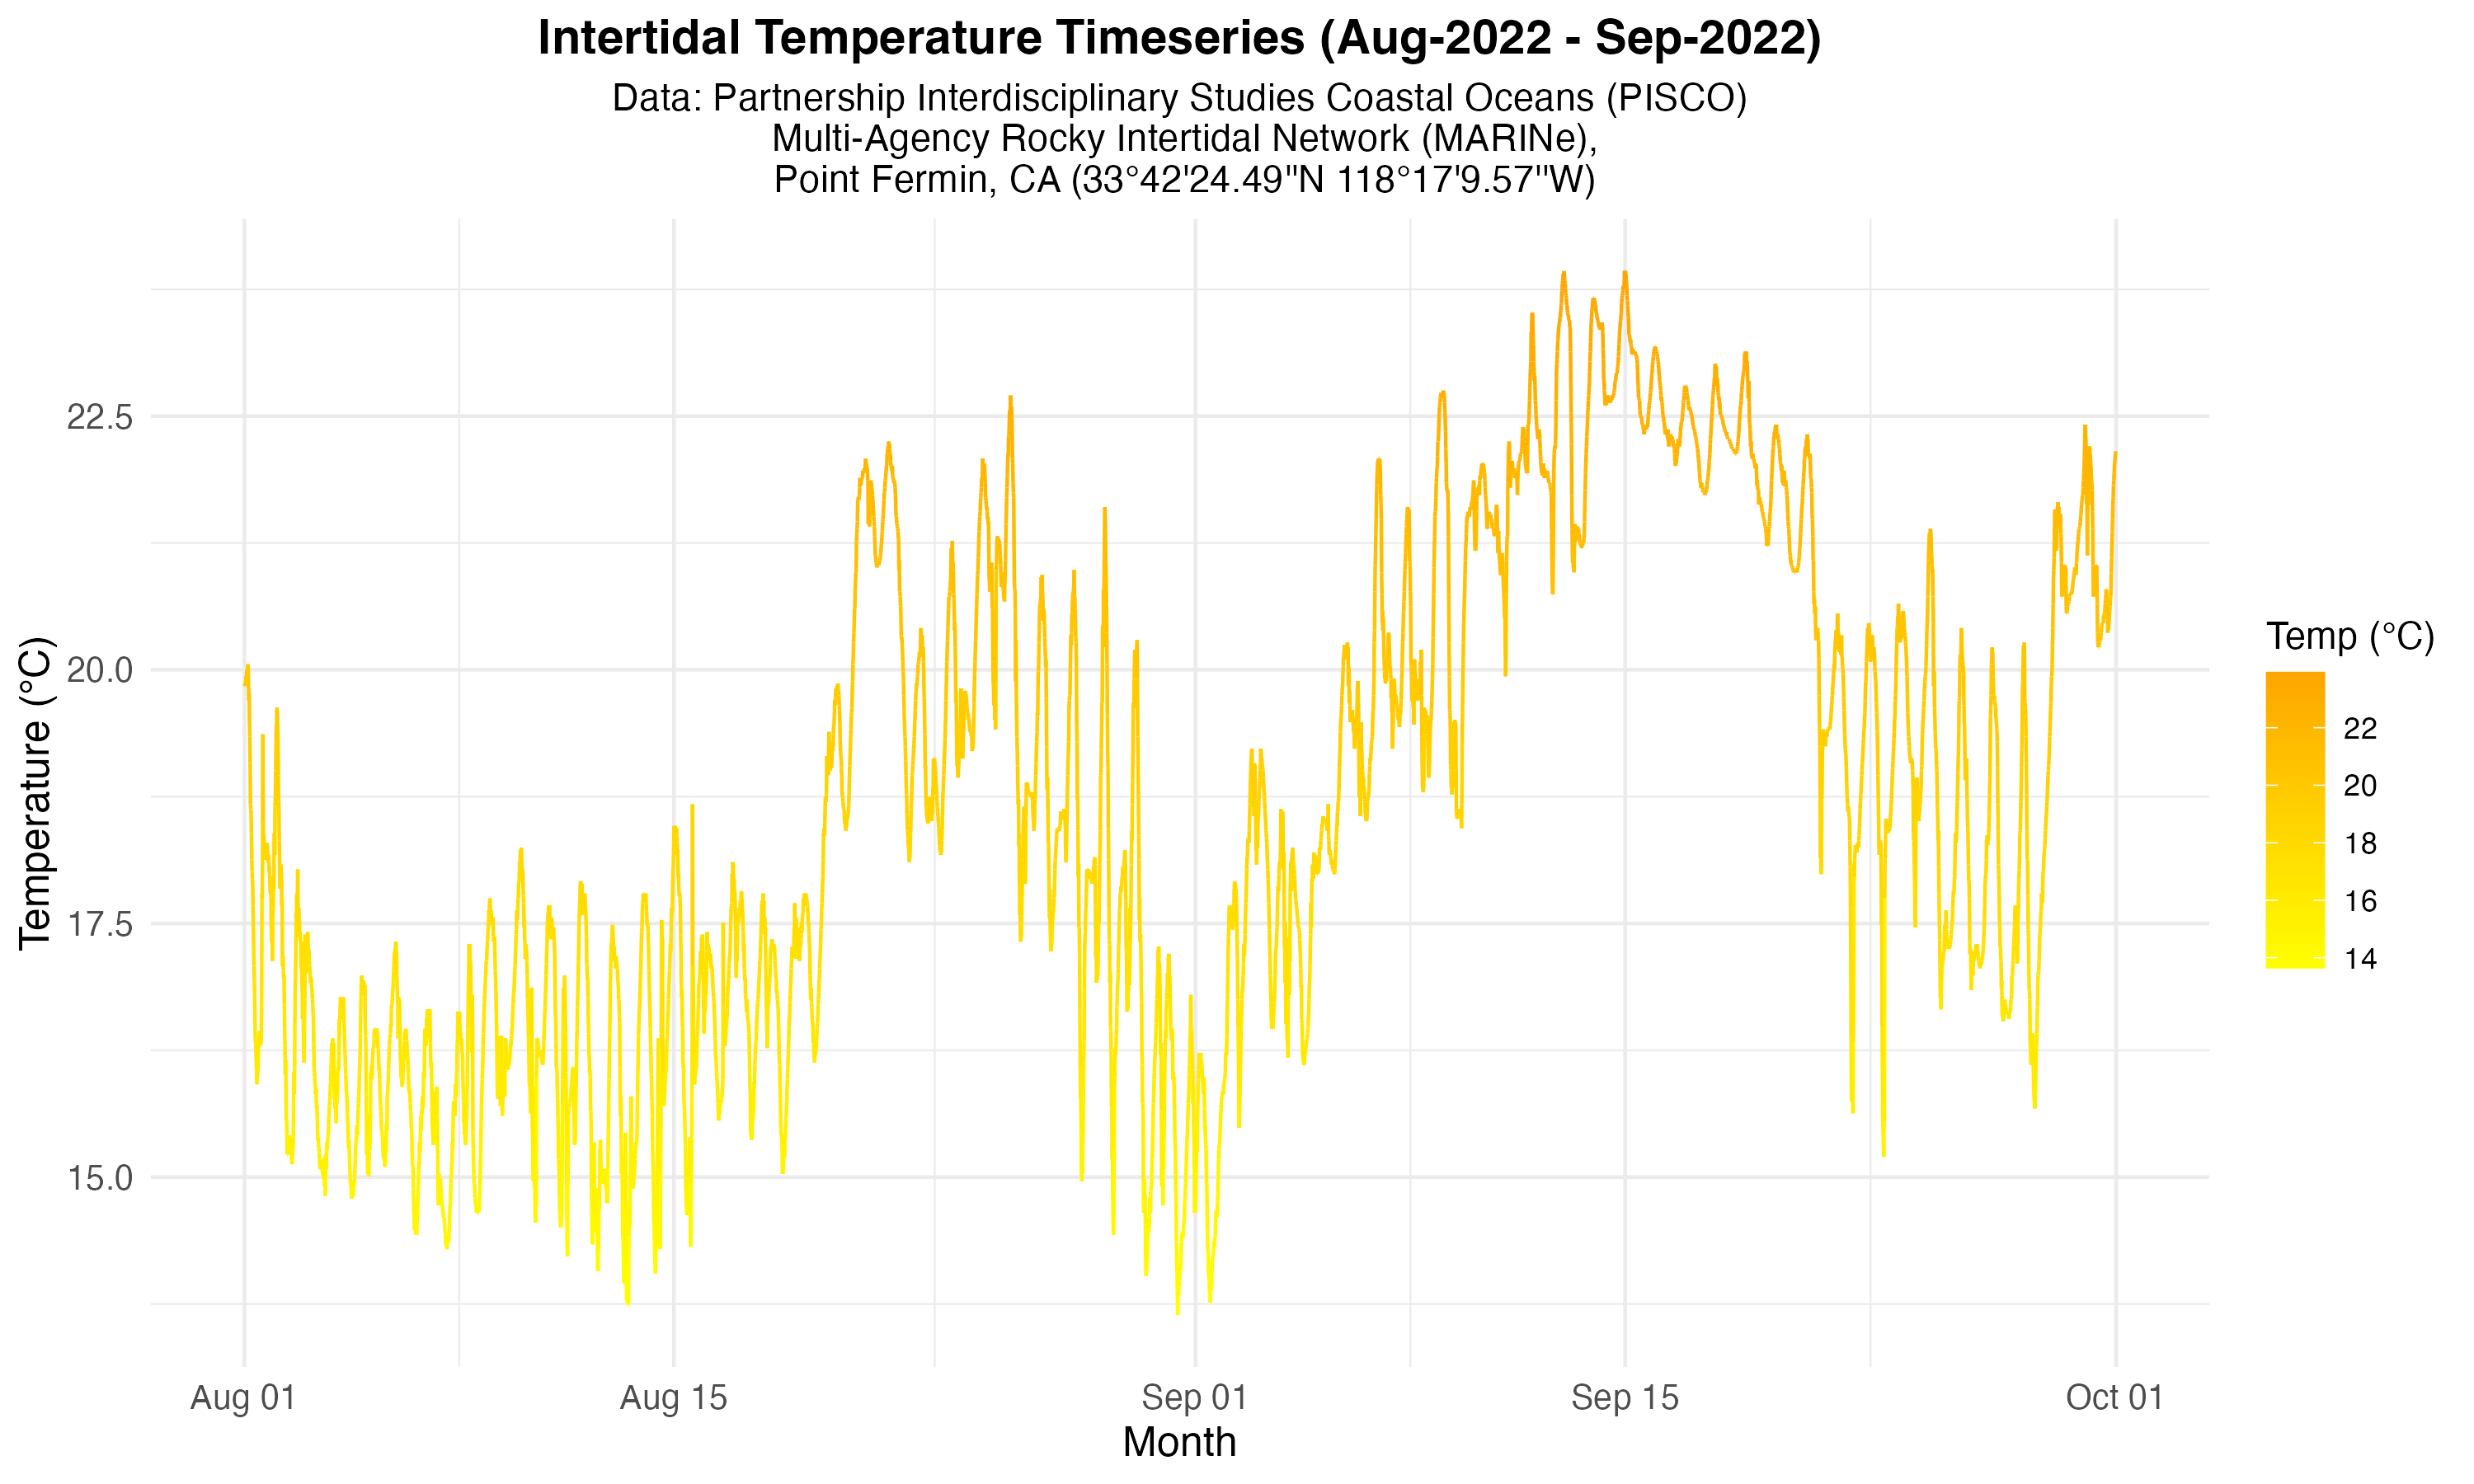
\includegraphics[width=0.8\textwidth]{Images/experiment_temp_timeseries_plot.png}
  \caption{Intertidal Temperature for Point Fermin, California (Data Collected Using: Onset Tidbit V2 Temp Data Logger) represented for August and September during the months of the experiment to visualize changes in SST. This figure zooms into the intertidal temperature dynamics during August and September, highlighting short-term fluctuations and potential impacts on intertidal organisms. Data sourced from the Multi-Agency Rocky Intertidal Network (MARINe) and Partnership Interdisciplinary Studies Coastal Oceans for of (PISCO) \citep{marine_pisco_burnaford_2023}.}
  \label{fig:intertidal-timeseries-zoom}
\end{figure}

\begin{figure}[htbp]
  \centering
  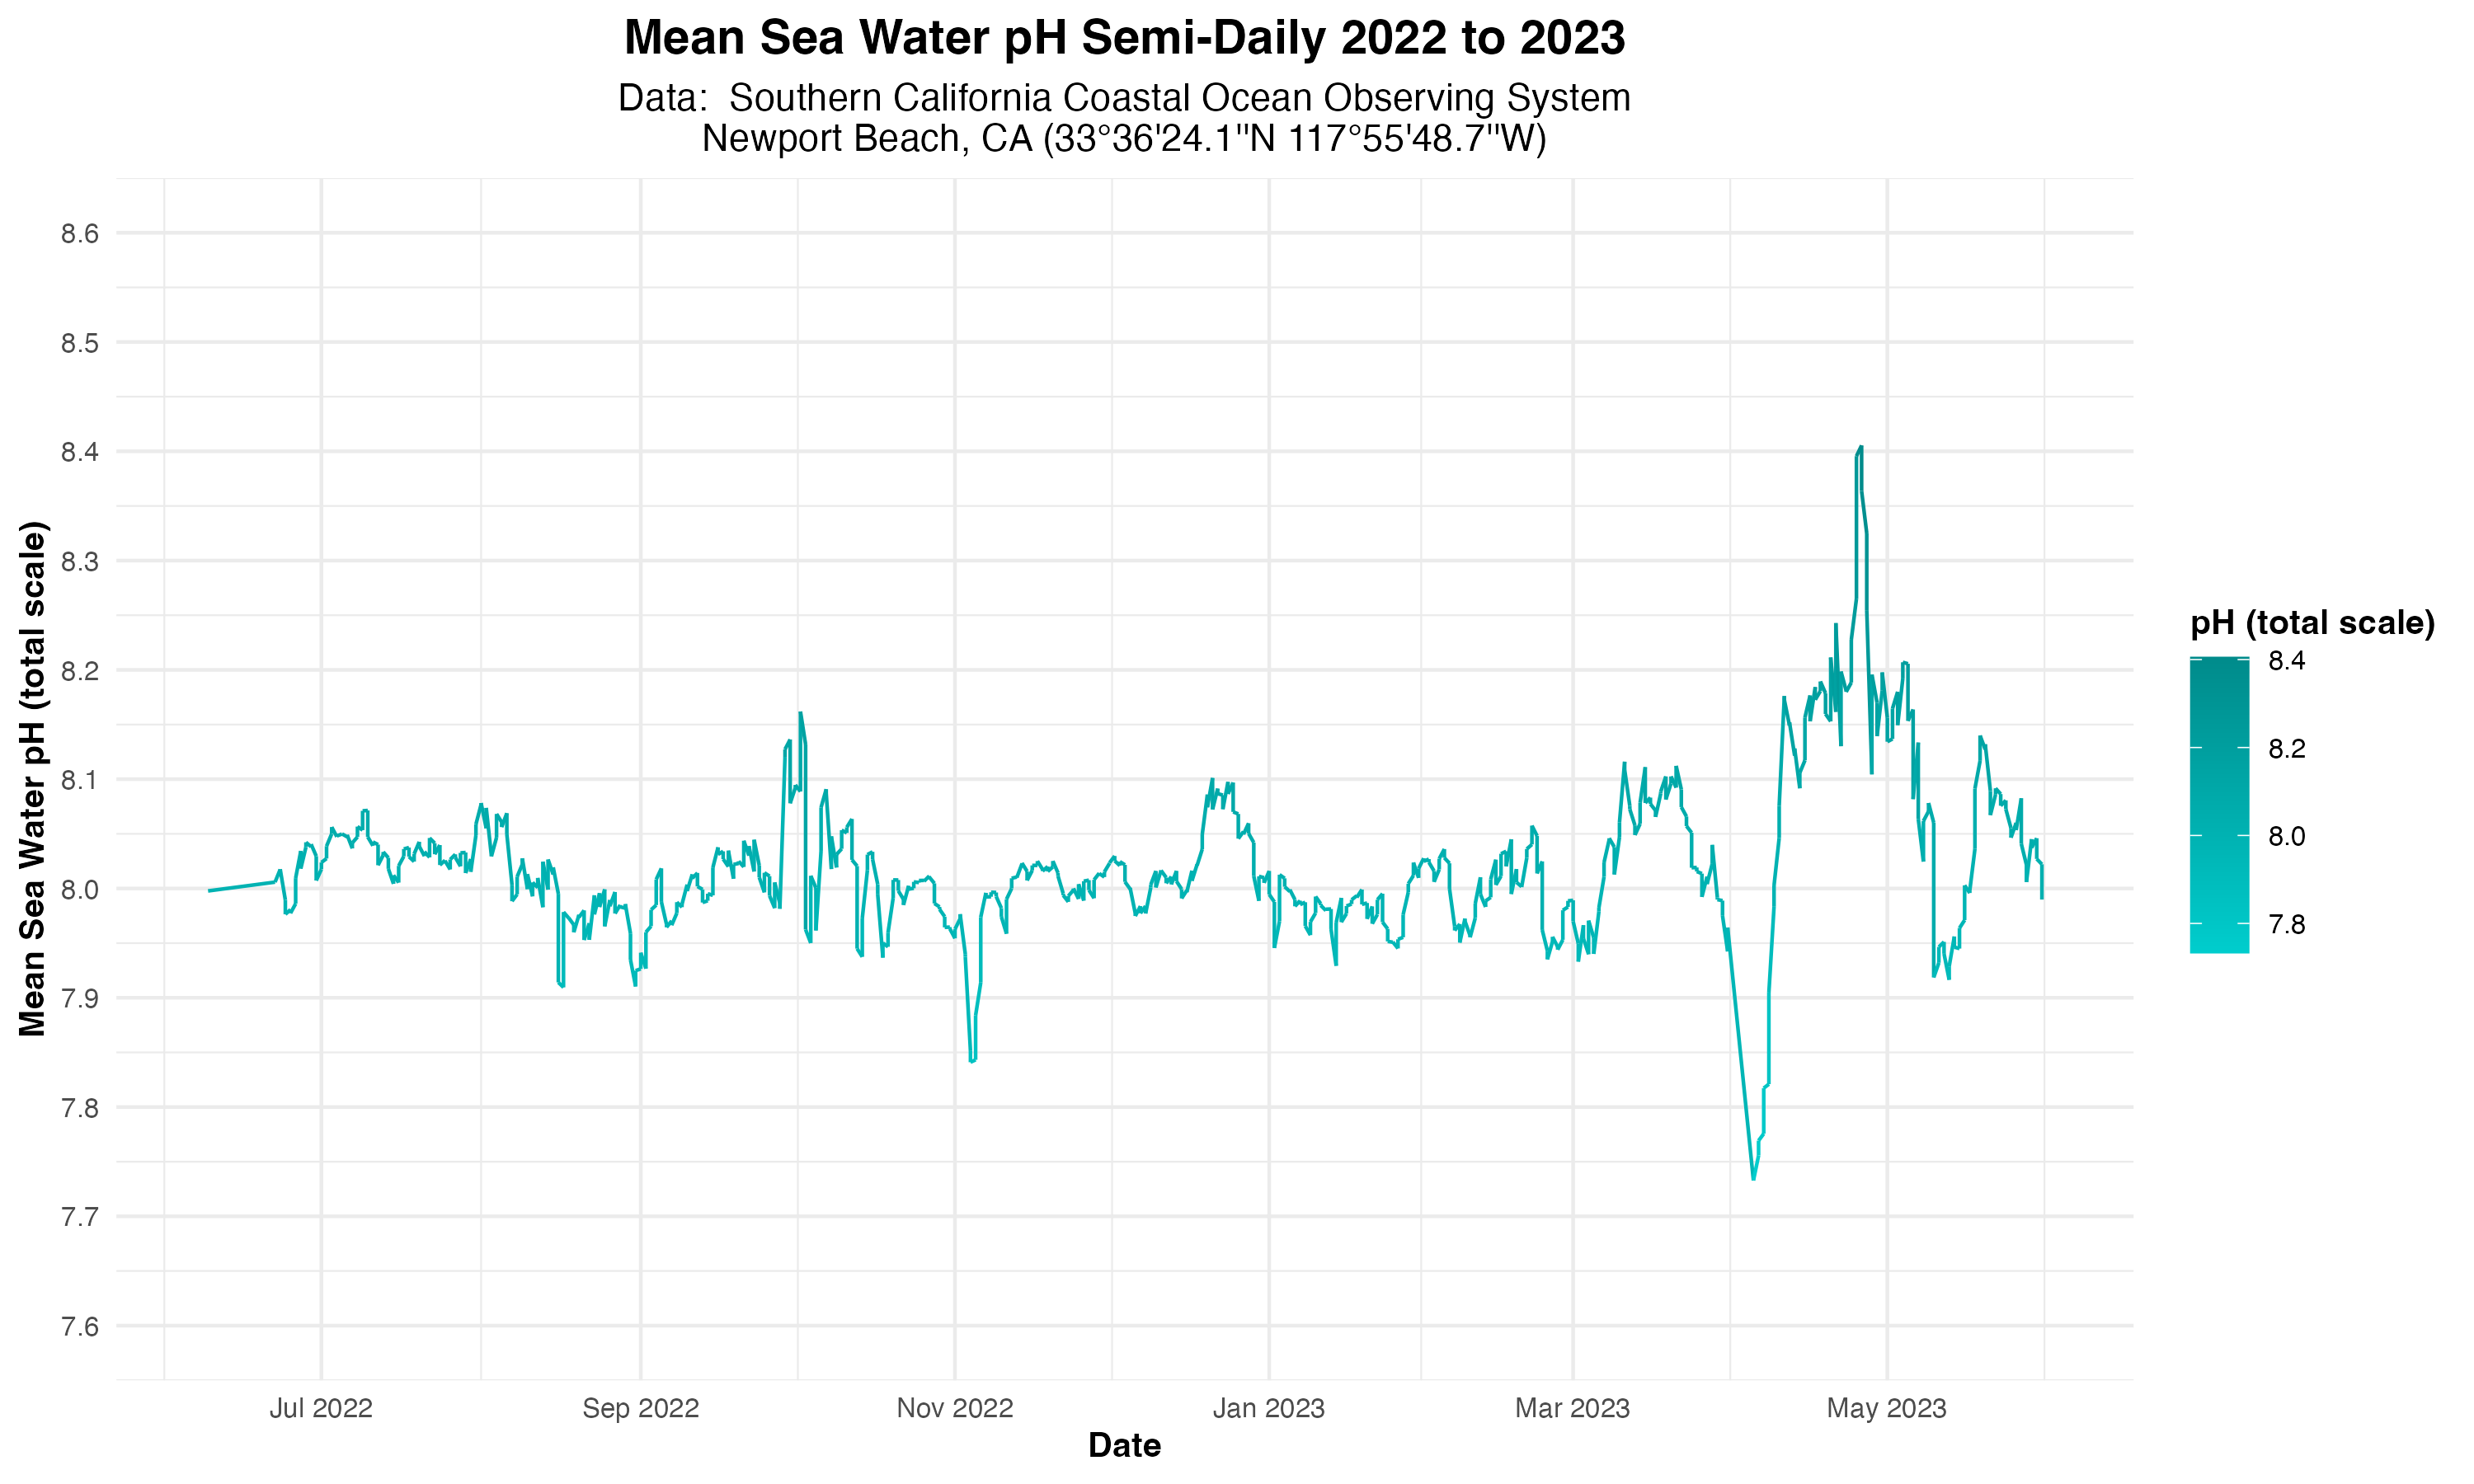
\includegraphics[width=0.8\textwidth]{Images/pH_timeseries_plot.png}
  \caption{Mean semi-daily pH (total scale) averaged every 12 hours for Newport Beach Pier in Newport, CA from 2022 to 2023. The data depict open ocean pH variability in an open shore environment without the drastic changes associated with changes in tide pool biogeochemistry. Data sourced from the Southern California Ocean Observing Systems (SCCOOS).}
  \label{fig:ph-timeseries}
\end{figure}

~~~~~ Sea snails were subjected to one of eight temperatures ranging
from 12-26\(^\circ\)C (12\(^\circ\)C, 14\(^\circ\)C, 16\(^\circ\)C,
18\(^\circ\)C, 20\(^\circ\)C, 22\(^\circ\)C, 24\(^\circ\)C,
26\(^\circ\)C; n=8) and either low or high pH conditions (7.7 or 8.0;
n=2), resulting in 16 experimental treatments. based on average facility
tank temperatures, or a realistic marine heatwave occurring on top of
ambient conditions. Nine tanks (three tanks per size class) underwent a
marine heatwave manipulation, while the remaining nine tanks were
maintained at ambient controls. Temperature conditions were chosen based
on sea surface temperature ranges and variability at a nearshore shore
station. pH was chosen due to the expected decreases of pH expected
under future conditions.

\hypertarget{d-survivorship}{%
\subsection{(d) Survivorship}\label{d-survivorship}}

~~~~~ Snail survivorship was monitored daily during the experiment.
Snails that exhibited signs of distress, such as being unable to adhere
to tank surfaces, being found at the bottom of the tank, or showing no
movement for a period of 24 hours, underwent sensory tests to assess
potential mortality. Specifically, snails were gently held w and touched
along their foot with forceps. If there was no response within thirty
seconds, they were considered deceased and subsequently removed from the
tank. Additionally, olfactory cues were also considered as indicators of
potential mortality.

\hypertarget{e-metabolic-experiment}{%
\subsection{(e) Metabolic Experiment}\label{e-metabolic-experiment}}

~~~~~ Respiration rates were measured after a 7-day adjustment period
and a 10-day exposure to the treatment conditions. Prior to conducting
respirometry, each individual snail shell was thoroughly scrubbed using
an acrylic brush to remove any epibiont communities that could
potentially obscure respiration rates. Snail respiration rates were
assessed by measuring oxygen evolution within sealed, water-tight
respirometry chambers (650 mL) for each individual. A mesh wire
separated the top and bottom sections of the chamber, with a magnetic
stir bar (200 rpms) placed in the bottom section to ensure proper mixing
of water and prevent oxygen stratification. During the respirometry
trials, temperature was carefully controlled and stabilized using an
insulated container and a programmable thermostat system (Apex
Controller, Neptune Systems \(\pm\) 0.1\(^\circ\) C). Temperature
adjustments were made using a submersible water heater (Finnex 300W
Titanium Heater) and a water chiller (Aqua Logic Delta Star, DS-4).
Oxygen measurements were taken at a frequency of 1 Hz using an oxygen
probe (Presens fiber optic oxygen dipping probe, DP-PSt8 \(\pm\)
0.1\(^\circ\) C) and continuously monitored throughout the 45-minute
respirometry trial using Presens Software. To ensure experimental
consistency, four organisms from each pH treatment (n= 8 snails) and one
blank control from each pH treatment (n = 2 blanks) were run together at
the same treatment temperature. This resulted in a total of 10
individual chambers placed in the respirometry stand and measured
simultaneously. Each chamber was fully submerged within the water bath
to maintain a controlled temperature inside. Since each respiration
chamber functioned as a sealed system, the oxygen consumption rate of
each individual organism (\((\mu mol \: O_2 \: g^{-1}h^{-1})\)) was
calculated and normalized to ash free dry weight. To obtain final wet
mass, snails were blotted with a paper towel to remove excess water,
scrubbed with a toothbrush to remove epibiont communities, and then
weighed using an electronic balance to the nearest 0.0001 g. Organic
biomass and ash free dry weight was obtained after the experiment,
during which snails were placed in a drying oven (Fisher Scientific
Isotemp Drying Oven) at 60\(^\circ\)C for 72 hours and then in a muffle
furnace (Fisher Scientific Isotemp Muffle Furnace) set to 450\(^\circ\)C
for 5 hours.

\hypertarget{f-statistical-analyses}{%
\subsection{(f) Statistical analyses}\label{f-statistical-analyses}}

~~~~~ To analyze the thermal performance curves of respiration rates and
determine the shape, we used the Sharpe Schoolfield high activation
energy model. statistical analysis was conducted in R software. The
Schoolfield model is widely used to describe the thermal performance
curves of biological rates of ectotherms. the Schoolfield model was
implemented in R to fit the data and estimate the parameters of the
model. The fitting process involved using the nmls and rTPC packages in
R to optimize the model parameters and estimate their uncertainty
\citep{padfield2021rtpc}. The data were fitted to the Sharpe Schoolfield
model (high) using AIC values between relevant performance models for
ectotherm species to evaluate the model's performance and the quality of
the fit. Furthermore, model selection techniques, such as comparing
different models based on their statistical criteria (e.g., AICc), were
employed to identify the most suitable model (e.g., gaussian,
sharpe-schoolfield low, sharpe-schoolfield full, sharpe-schoolfield
high, weibull) that accurately described the observed thermal
performance curve. Furthermore, I conducted bootstrap resampling to
estimate confidence intervals for the model predictions.

\end{document}
